\documentclass[12pt]{article}

\usepackage[margin=1in]{geometry} 
\usepackage{amsmath,amsthm,amssymb,scrextend}
\usepackage{fancyhdr}
\pagestyle{fancy}
\usepackage{xcolor}
\usepackage{pgfplots}
\usepackage{enumitem}
\pgfplotsset{compat=1.18}

\newcommand{\N}{\mathbb{N}}
\newcommand{\Z}{\mathbb{Z}}
\newcommand{\I}{\mathbb{I}}
\newcommand{\R}{\mathbb{R}}
\newcommand{\Q}{\mathbb{Q}}
\renewcommand{\qed}{\hfill$\blacksquare$}
\let\newproof\proof
\renewenvironment{proof}{\begin{addmargin}[1em]{0em}\begin{newproof}}{\end{newproof}\end{addmargin}\qed}
% \newcommand{\expl}[1]{\text{\hfill[#1]}$}

\newenvironment{theorem}[2][Theorem]{\begin{trivlist}
		\item[\hskip \labelsep {\bfseries #1}\hskip \labelsep {\bfseries #2.}]}{\end{trivlist}}
\newenvironment{lemma}[2][Lemma]{\begin{trivlist}
		\item[\hskip \labelsep {\bfseries #1}\hskip \labelsep {\bfseries #2.}]}{\end{trivlist}}
\newenvironment{problem}[2][Problem]{\begin{trivlist}
		\item[\hskip \labelsep {\bfseries #1}\hskip \labelsep {\bfseries #2.}]}{\end{trivlist}}
\newenvironment{exercise}[2][Exercise]{\begin{trivlist}
		\item[\hskip \labelsep {\bfseries #1}\hskip \labelsep {\bfseries #2.}]}{\end{trivlist}}
\newenvironment{reflection}[2][Reflection]{\begin{trivlist}
		\item[\hskip \labelsep {\bfseries #1}\hskip \labelsep {\bfseries #2.}]}{\end{trivlist}}
\newenvironment{proposition}[2][Proposition]{\begin{trivlist}
		\item[\hskip \labelsep {\bfseries #1}\hskip \labelsep {\bfseries #2.}]}{\end{trivlist}}
\newenvironment{corollary}[2][Corollary]{\begin{trivlist}
		\item[\hskip \labelsep {\bfseries #1}\hskip \labelsep {\bfseries #2.}]}{\end{trivlist}}

\setlength{\parindent}{0pt}

\begin{document}
	% for only the first page and for all the pages for pdf version
	\fancyhf{}
	\lhead{Formulas}
	\section*{Some Taylor / Maclaurin  Series Formulas}

	\[\boldsymbol{f(x)} = \sum_{n=0}^{\infty} \frac{f^{(n)}(a)}{n!}(x-a)^n = f(a) + f'(a)(x-a) + \frac{f''(a)}{2!}(x-a)^2 + \cdots\]

	When $a=0$, it is Maclaurin series:

	\[\boldsymbol{f(x)} = \sum_{n=0}^{\infty} \frac{f^{(n)}(0)}{n!}x^n = f(0) + f'(0)x + \frac{f''(0)}{2!}x^2 + \frac{f'''(0)}{3!}x^3 + \cdots\]

	\[\begin{aligned}
		\boldsymbol{e^{x}}&=\sum_{n=0}^{\infty} \frac{1}{n !} x^{n}=1+x+\frac{1}{2 !} x^{2}+\cdots, \quad x \in(-\infty,+\infty) \\[1ex]
		\boldsymbol{\sin x}&=\sum_{n=0}^{\infty} \frac{(-1)^{n}}{(2 n+1) !} x^{2 n+1}=x-\frac{1}{3 !} x^{3}+\frac{1}{5 !} x^{5}+\cdots,\quad x \in(-\infty,+\infty) \\[1ex]
		\boldsymbol{\cos x}&=\sum_{n=0}^{\infty} \frac{(-1)^{n}}{(2 n) !} x^{2 n}=1-\frac{1}{2 !} x^{2}+\frac{1}{4 !} x^{4}+\cdots,\quad  x \in(-\infty,+\infty) \\[1ex]
		\boldsymbol{\ln (1+x)}&=\sum_{n=0}^{\infty} \frac{(-1)^{n}}{n+1} x^{n+1}=x-\frac{1}{2} x^{2}+\frac{1}{3} x^{3}+\cdots,\quad  x \in(-1,1] \\[1ex]
		\boldsymbol{\frac{1}{1-x}}&=\sum_{n=0}^{\infty} x^{n}=1+x+x^{2}+x^{3}+\cdots,\quad  x \in(-1,1) \\[1ex]
		\boldsymbol{\frac{1}{1+x}}&=\sum_{n=0}^{\infty}(-1)^{n} x^{n}=1-x+x^{2}-x^{3}+\cdots,\quad  x \in(-1,1)\\[1ex]
		\boldsymbol{(1+x)^{\alpha}}&=1+\sum_{n=1}^{\infty} \frac{\alpha(\alpha-1) \cdots(\alpha-n+1)}{n !} x^{n}=1+\alpha x+\frac{\alpha(\alpha-1)}{2 !} x^{2}+\cdots,\quad  x \in(-1,1) \\[1ex]
		\boldsymbol{\arctan x}&=\sum_{n=0}^{\infty} \frac{(-1)^{n}}{2 n+1} x^{2 n+1}=x-\frac{1}{3} x^{3}+\frac{1}{5} x^{5}+\cdots,\quad  x \in[-1,1] \\[1ex]
		\boldsymbol{\arcsin x}&=\sum_{n=0}^{\infty} \frac{(2 n) !}{4^{n}(n !)^{2}(2 n+1)} x^{2n+1}=x+\frac{1}{6} x^{3}+\frac{3}{40} x^{5}+\frac{5}{112} x^{7}+\frac{35}{1152} x^{9}+\cdots,\quad  x \in(-1,1)\\[1ex]
		\boldsymbol{\tan x}&=\sum_{n=1}^{\infty} \frac{B_{2 n}(-4)^{n}\left(1-4^{n}\right)}{(2 n) !} x^{2 n-1}=x+\frac{1}{3} x^{3}+\frac{2}{15} x^{5}+\frac{17}{315} x^{7}+\frac{62}{2835} x^{9}+\cdots,\quad x\in (-\frac{\pi}{2},\frac{\pi}{2})
	\end{aligned}\]
	\newpage

	\section*{Hyperbolic Trigonometric Identities}
	$$
	\sinh x = \frac{e^x - e^{-x}}{2}
	$$
	
	$$
	\cosh x = \frac{e^x + e^{-x}}{2}
	$$
	
	$$
	\tanh x = \frac{\sinh x}{\cosh x} = \frac{e^x - e^{-x}}{e^x + e^{-x}}
	$$

	\begin{center}
	\begin{tikzpicture}
	\begin{axis}[
		width=0.9\textwidth,
		height=0.32\textheight,
		xmin=-5, xmax=5,
		ymin=-3, ymax=3,
		axis lines=middle,
		xlabel={$x$},
		ylabel={$y$},
		ylabel style={at={(axis description cs:0.5,1.02)},anchor=south},
		xtick=\empty,
		ytick=\empty,
		xticklabels={},
		yticklabels={},
		axis equal image=true,
		legend style={at={(0.98,0.02)},anchor=south east,fill=white},
		samples=200
	]
	\addplot[red, thick] {sinh(x)};
	\addlegendentry{$\sinh x$}
	\addplot[blue, thick] {cosh(x)};
	\addlegendentry{$\cosh x$}
	\addplot[green!40!black, thick] {tanh(x)};
	\addlegendentry{$\tanh x$}
	\end{axis}
	\end{tikzpicture}
	\end{center}
	
	$$
	\coth x = \frac{\cosh x}{\sinh x} = \frac{e^x + e^{-x}}{e^x - e^{-x}}
	\qquad \text{for } x \ne 0
	$$
	
	$$
	\operatorname{sech} x = \frac{1}{\cosh x} = \frac{2}{e^x + e^{-x}}
	$$
	
	$$
	\operatorname{csch} x = \frac{1}{\sinh x} = \frac{2}{e^x - e^{-x}}
	\qquad \text{for } x \ne 0
	$$

	\begin{center}
	\begin{tikzpicture}
	\begin{axis}[
		width=0.9\textwidth,
		height=0.32\textheight,
		xmin=-5, xmax=5,
		ymin=-3, ymax=3,
		axis lines=middle,
		xlabel={$x$},
		ylabel={$y$},
		ylabel style={at={(ticklabel* cs:1.05)},anchor=center},
		xtick=\empty,
		ytick=\empty,
		xticklabels={},
		yticklabels={},
		axis equal image=true,
		legend style={at={(0.98,0.02)},anchor=south east,fill=white},
		samples=200
	]
	\addplot[red, thick, domain=-5:-0.08] {cosh(x)/sinh(x)};
	\addplot[red, thick, domain=0.08:5, forget plot] {cosh(x)/sinh(x)};
	\addlegendentry{$\coth x$}
	\addplot[blue, thick, domain=-5:5] {1/cosh(x)};
	\addlegendentry{$\operatorname{sech} x$}
	\addplot[green!40!black, thick, domain=-5:-0.08] {1/sinh(x)};
	\addplot[green!40!black, thick, domain=0.08:5, forget plot] {1/sinh(x)};
	\addlegendentry{$\operatorname{csch} x$}
	\end{axis}
	\end{tikzpicture}
	\end{center}
	
	\newpage

	\section*{Trigonometric Identities}

	\[
	\begin{aligned}
		\sin^2 x+\cos^2 x&=1 \\[0.5ex]
		1+\tan^2 x&=\sec^2 x \\[0.5ex]
		1+\cot^2 x&=\csc^2 x
	\end{aligned}
	\]

	\[
	\begin{aligned}
		\sin(A+B)&=\sin A\cos B+\cos A\sin B \\[0.5ex]
		\sin(A-B)&=\sin A\cos B-\cos A\sin B \\[0.5ex]
		\cos(A+B)&=\cos A\cos B-\sin A\sin B \\[0.5ex]
		\cos(A-B)&=\cos A\cos B+\sin A\sin B \\[0.5ex]
		\tan(A+B)&=\frac{\tan A+\tan B}{1-\tan A\tan B} \\[0.5ex]
		\tan(A-B)&=\frac{\tan A-\tan B}{1+\tan A\tan B}
	\end{aligned}
	\]

	\[
	\begin{aligned}
		\sin 2x&=2\sin x\cos x \\[0.5ex]
		\cos 2x&=\cos^2 x-\sin^2 x=2\cos^2 x-1=1-2\sin^2 x \\[0.5ex]
		\tan 2x&=\frac{2\tan x}{1-\tan^2 x}
	\end{aligned}
	\]

	\[
	\begin{aligned}
		\sin^2 \frac{x}{2}&=\frac{1-\cos x}{2} \\[0.5ex]
		\cos^2 \frac{x}{2}&=\frac{1+\cos x}{2} \\[0.5ex]
		\tan \frac{x}{2}&=\frac{\sin x}{1+\cos x}=\frac{1-\cos x}{\sin x}
	\end{aligned}
	\]

	\[
	\begin{aligned}
		\sin A+\sin B&=2\sin \frac{A+B}{2}\cos \frac{A-B}{2} \\[0.5ex]
		\sin A-\sin B&=2\cos \frac{A+B}{2}\sin \frac{A-B}{2} \\[0.5ex]
		\cos A+\cos B&=2\cos \frac{A+B}{2}\cos \frac{A-B}{2} \\[0.5ex]
		\cos A-\cos B&=-2\sin \frac{A+B}{2}\sin \frac{A-B}{2}
	\end{aligned}
	\]

	\[
	\begin{aligned}
		2\sin A\cos B&=\sin(A+B)+\sin(A-B) \\[0.5ex]
		2\cos A\cos B&=\cos(A+B)+\cos(A-B)
	\end{aligned}
	\]

	\[
	\begin{aligned}
		\sec x&=\frac{1}{\cos x}, \qquad \csc x=\frac{1}{\sin x}, \qquad \cot x=\frac{\cos x}{\sin x} \\[0.5ex]
		\sin\left(\frac{\pi}{2}-x\right)&=\cos x, \qquad \cos\left(\frac{\pi}{2}-x\right)=\sin x, \qquad \tan\left(\frac{\pi}{2}-x\right)=\cot x
	\end{aligned}
	\]

	\newpage

	\section*{Hyperbolic Functions}

	\[
	\cosh^2 x-\sinh^2 x=1
	\]

	\[
	\sinh 2x=2\sinh x\cosh x
	\]

	\[
	\cosh 2x=\cosh^2 x+\sinh^2 x
	\]

	\[
	\cosh^{-1}x=\ln\!\left(x+\sqrt{x^2-1}\right)\qquad (x\ge 1)
	\]

	\[
	\sinh^{-1}x=\ln\!\left(x+\sqrt{x^2+1}\right)
	\]

	\[
	\tanh^{-1}x=\frac{1}{2}\ln\!\left(\frac{1+x}{1-x}\right)\qquad (|x|<1)
	\]

	\[
	\begin{aligned}
		\int \operatorname{sech}^2 x\,\mathrm{d}x&=\tanh x+C \\[0.5ex]
		\int \operatorname{csch}^2 x\,\mathrm{d}x&=-\coth x+C \\[0.5ex]
		\int \operatorname{sech} x\tanh x\,\mathrm{d}x&=-\operatorname{sech} x+C \\[0.5ex]
		\int \operatorname{csch} x\coth x\,\mathrm{d}x&=-\operatorname{csch} x+C
	\end{aligned}
	\]

	\[
	\begin{aligned}
		\int \frac{1}{\sqrt{x^2+1}}\,\mathrm{d}x&=\sinh^{-1}x+C \\[0.5ex]
		\int \frac{1}{\sqrt{x^2-1}}\,\mathrm{d}x&=\cosh^{-1}x+C \qquad (x>1) \\[0.5ex]
		\int \frac{1}{1-x^2}\,\mathrm{d}x&=\tanh^{-1}x+C \qquad (|x|<1)
	\end{aligned}
	\]

	\newpage

	\section*{Algebraic Identities}

	\[
	a^2-b^2=(a+b)(a-b)
	\]

	\[
	a^2+2ab+b^2=(a+b)^2
	\]

	\[
	a^2-2ab+b^2=(a-b)^2
	\]

	\[
	a^3+b^3=(a+b)(a^2-ab+b^2)
	\]

	\[
	a^3-b^3=(a-b)(a^2+ab+b^2)
	\]

	\[
	a^3+3a^2b+3ab^2+b^3=(a+b)^3
	\]

	\[
	a^3-3a^2b+3ab^2-b^3=(a-b)^3
	\]

	\[
	a^4-b^4=(a-b)(a+b)(a^2+b^2)
	\]

	\[
	a^n-b^n=(a-b)(a^{n-1}+a^{n-2}b+\cdots+ab^{n-2}+b^{n-1})
	\]

	\[
	(a+b+c)^2=a^2+b^2+c^2+2ab+2ac+2bc
	\]

	\[
	x^2-(a+b)x+ab=(x-a)(x-b)
	\]

	\[
	\frac{1}{a}+\frac{1}{b}=\frac{a+b}{ab}
	\]

	\[
	\frac{1}{a-b}-\frac{1}{a+b}=\frac{2b}{a^2-b^2}
	\]

	\newpage

	\section*{Differentiation and Integration}

	\[
	\begin{aligned}
		\frac{\mathrm{d}}{\mathrm{d}x}(uv)&=u'v+uv' \\[0.5ex]
		\frac{\mathrm{d}}{\mathrm{d}x}\left(\frac{u}{v}\right)&=\frac{u'v-uv'}{v^2} \\[0.5ex]
		\frac{\mathrm{d}}{\mathrm{d}x}\bigl(f(g(x))\bigr)&=f'(g(x))g'(x)
	\end{aligned}
	\]

	\[
	\begin{aligned}
		\int \frac{1}{a^2+x^2}\,\mathrm{d}x&=\frac{1}{a}\arctan\frac{x}{a}+C
	\end{aligned}
	\]

	\[
	\int u'v\,\mathrm{d}x=uv-\int uv'\,\mathrm{d}x
	\]

	\[
	\int_a^b f(g(x))g'(x)\,\mathrm{d}x=\int_{g(a)}^{g(b)} f(u)\,\mathrm{d}u
	\]

	\[
		\int_a^b f'(x)\,\mathrm{d}x=f(b)-f(a)
	\]

	\newpage

	\[
	\operatorname{Var}(X)=E\bigl((X-\mu)^2\bigr)=E(X^2)-\mu^2
	\]

	\[
	\operatorname{Cov}(X,Y)=E\bigl((X-\mu_X)(Y-\mu_Y)\bigr)=E(XY)-\mu_X\mu_Y
	\]

	\[
	\operatorname{Var}(aX\pm bY)=a^2\operatorname{Var}(X)+b^2\operatorname{Var}(Y)\pm 2ab\,\operatorname{Cov}(X,Y)
	\]

	\[
	\rho=\frac{\operatorname{Cov}(X,Y)}{\sigma_X\sigma_Y}
	\]

	For independent random variables $X$ and $Y$:
	\[
	E(XY)=E(X)E(Y)
	\]
	\[
	\operatorname{Var}(aX\pm bY)=a^2\operatorname{Var}(X)+b^2\operatorname{Var}(Y)
	\]

	\newpage

	\section*{Common Cumulative Distribution Functions (CDFs)}

	The CDF of a random variable \(X\) is \(F_X(x)=P(X\le x)\).

	The PDF of a random variable \(X\) is \(f_X(x)=F_X'(x)\).

	When $X\sim N(\mu,\sigma^2):$
	\[
	F_X(x)=\frac{1}{\sqrt{2\pi}}\int_{-\infty}^{\frac{x-\mu}{\sigma}} e^{-t^2/2}\,\mathrm{d}t
	\qquad
	f_X(x)=\frac{1}{\sigma\sqrt{2\pi}}e^{-\frac{(x-\mu)^2}{2\sigma^2}}
	\]

	When $X\sim \mathrm{Bin}(n,p):$
	\[
	F_X(x)=\sum_{r=0}^{\lfloor x\rfloor}\binom{n}{r}p^r(1-p)^{n-r}
	\qquad
	P_X(x)=\binom{n}{x}p^x(1-p)^{n-x}
	\]

	When $X\sim \mathrm{Geo}(p):$
	\[
	F_X(x)=\sum_{r=1}^{\lfloor x\rfloor}p(1-p)^{r-1}
	\qquad
	P_X(x)=p(1-p)^{x-1}
	\]

	When $X\sim \mathrm{Po}(\lambda):$
	\[
	F_X(x)=e^{-\lambda}\sum_{r=0}^{\lfloor x\rfloor}\frac{\lambda^r}{r!}
	\qquad
	P_X(x)=e^{-\lambda}\frac{\lambda^x}{x!}
	\]

	\newpage
	
	\subsection*{e}
	\[
	\begin{aligned}
	e&=\lim_{n\to\infty}\left(1+\frac{1}{n}\right)^n\\
	&=\sum_{n=0}^{\infty}\frac{1}{n!}\\
	&=1+1+\frac{1}{2!}+\frac{1}{3!}+\cdots
	\end{aligned}
	\]


\end{document}
